\chapter{The Design and Development of the Immotion Exergame}\label{chapter:implementation}

This chapter outlines the design and development of the Immotion exergame for warm up routine guidance and motivation. We begin with the description of the design methodology used for the development. For the purpose of this thesis, an iterative and prototype driven, user centered design has been adopted (UCD). Particular needs of individuals who engage in some sort of physical (sports) activity has been gathered through the adopted UCD process in order to make an adequate exergames for warm up guidance and motivation. We chose the \textit{Spiral model} as our chosen exergame development model. \\\\ Next, we cover the main development iterations that have been undertaken during the exergame design and development process. 

\section{Overview of User Centered Design}
The theory of UCD is ensuring that the user's needs and goals are the primary consideration at every stage of the development (Norman 1990).

Below are the general phases of User-Centered Design process:[11][12] wiki
Specify context of use: Identify who the primary users of the product, why they will use the product, what are their requirements and under what environment they will use it.
Specify Requirements: Once the context is specified, it is the time to identify the granular requirements of the product. This is an important process which can further facilitate the designers to create storyboards, and set important goals to make the product successful.
Create Design solutions and development: Based on product goals and requirements, start an iterative process of product design and development.
Evaluate Product: Product designers do usability testing to get users' feedback of the product.Product evaluation is a crucial step in product development which gives critical feedback of the product.[13]
In the next steps, the above procedure is repeated to further finish the product. 

\section{The Context of Use}
There are solutions designed to encourage physical activity.
Identify the people who will use the product, what they will use it for, and under what conditions they will use it.
\section{Overview of the Development Phases}
The development of the Immotion exergame consisted of three primary phases which are according to the well accepted game design phases outlined by Furher and are depicted in Figure \ref{fig:iterations}: 
\begin{itemize}
\item Requirements gathering 
\item First prototype development with user evaluation
\item Final exergame development with further user evaluation
\end{itemize}
In the following sections, each iteration presented in Development section of Figure \ref{fig:iterations} will be further detailed. 

\begin{figure}[h]
    \centering
    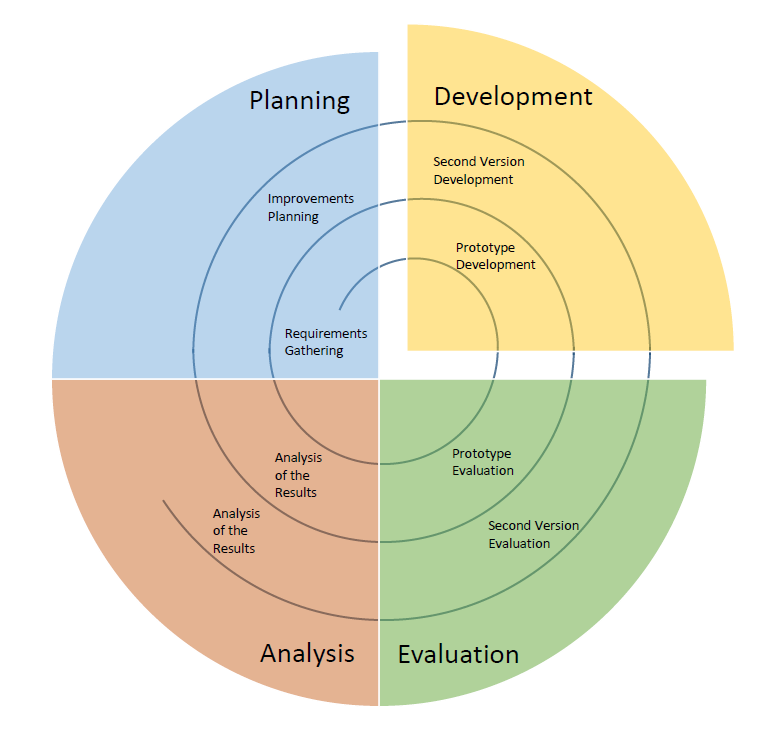
\includegraphics[width=\textwidth]{iterations}
    \caption{Overview of the development iterations}
    \label{fig:iterations}
\end{figure}
\subsection{Requirements Gathering}
This iteration was an exploratory step that justified the development and identified the currently available solutions in the domain of exergames for warm up before sports activities. This was achieved through initial literature review related to exergame, gamification and motivational psychology which identified the most important areas to be addressed when developing gamified solution in the given context. Furthermore, in order to design an enjoyable gaming solution for warm up guidance and motivation, several warm up and sports related requirements needed to be considered too. Having this in mind, sports and fitness related literature have been reviewed as well. Particular attention has been put on those warm up exercises that could hypothetically help in injury prevention, improvement performance, and could be included in our solution as one of the required movement. The selected movements should increase core temperature, blood flow, and prepare the body for the subsequent exercise.\\ As previously pointed out, the exergame is meant to be used in a gym or fitness centers before physically demanding sports activity. Having this in mind, the set of movements that required in the game had do be carefully selected. Some of the requirements were as follows:
\begin{itemize}
\item Movements need to be easily detectable by only one Kinect device.
\item Movements should be easy enough to be correctly performed without any prior knowledge of the movement.
\item Only movements that can be executed without additional equipment should to be considered.   
\item Only movements recommended for the general warm up routines outlined in sports related literature and suggested by experts should be considered.
\item The duration of the exergame guided warm up routine should correspond to the warm up duration suggested by sports literature and experts.
\end{itemize}
%http://assets.ngin.com/attachments/document/0035/1162/FIFA_11__EXERCISES.pdf
%https://www.kort.com/uploadedFiles/KORT/Content/Services/Sports_Medicine/Concussion_Management/FIFA-the-11-Booklet.pdf
Since no well documented and medically supported warm up programmes for workout routines were found,  the required movements were adopted from the 
\textit{FIFA 11}[] and \textit{FIFA 11+}[] warm up programmes which mostly focus on core and leg strength, balance, and agility. These programmes were shown to have significant impact on injury reduction in football players and can lead to improvements in thigh muscle strength, jump height, and sprint speed [].%https://www.ncbi.nlm.nih.gov/pmc/articles/PMC4245655/
Based on the mentioned warm up programmes review, taking into account the requirements and hardware restrictions, the following movements were found to be suitable for the prototype solution: 
\begin{itemize}
\item jump right,
\item jump left,
\item jump up, and
\item squat.
\end{itemize}
After the requirements were specified and the required movements selected, we start with the prototype development phase.
\subsection{Prototype Development}
This section outlines the development of the prototype version of the exergame for warm up before sports activities. Our primary goal was to develop a working version of the exergame that can process movements in real time in order to guide users through the warm up routine and, presumably, immerses the participants sufficiently so that their focus is shifted from the discomfort and exertion of the exercise towards the enjoyment of the experience. The prototype was developed as a scaled down version of our planned final solution. With the prototype, we aimed to learn more about the problem, possible target groups, and explore the most suitable design and implementation techniques that could be used during the exergame development process. 
\subsubsection{Game Description}
The Immotion exergame has been created using the Unity 5.6 game development platform developed by Unity Technologies []. User's movements were captured and processed using Kinect for Xbox One (2.0 2013) motion sensing input devices by Microsoft []. The game engine was run on XX [] and projected on a wall using XX projector. In figure \ref{fig:hs} we outline the relationship of the game, software, and hardware equipment.\\
\begin{figure}[h]
    \centering
    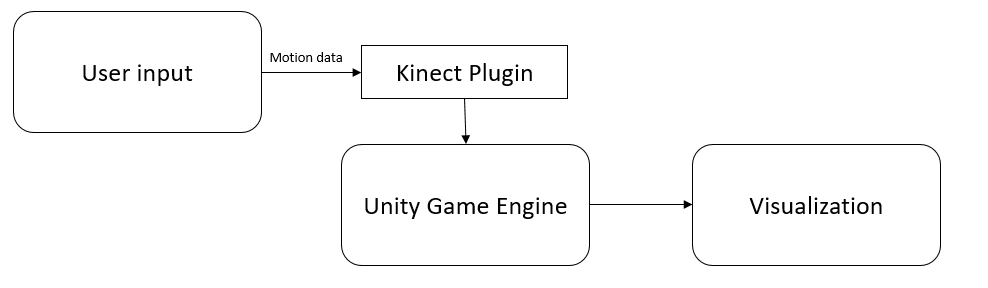
\includegraphics[width=\textwidth]{hardware_software}
    \caption{Hardware and Software supporting the prototype exergame}
    \label{fig:hs}
\end{figure}\\
For the prototype version of the exergame, a game scenario that is similar to Subway Surfers [] and Temple Run [] games has been implemented. In these games, the player controls the character that is on a track and needs to move left, right or jump up in order to avoid obstacles and collect points. In our solution, the player controls the character by doing a set of movements, which are tracked using a Microsoft Kinect device. In-game obstacles (e.i. walls or boxes) and coins were positioned in a way that the user is required to perform a specific movement in order to avoid the obstacle or collect a coin. By collecting coins the overall user score was increased. Contrarily, by hitting an obstacle, the overall user score was decreased. By placing the obstacle and coins in a specific position, our intention was to indirectly promote exercise through the gameplay of repeatedly performing warm up related movements chosen during the Gathering Requirements phase.

\subsubsection{Gamification Elements}
In order to create an immersive game environment that will shift users' focus from the exertion of the exercise, we also employ few game \textit{mechanics}.  Werbach and Hunter [] (2012) report that mechanics provide the ''\textit{basic processes that drive the action forward and generate
player engagement}''. For the prototype version of the Immotion exergame, the most important mechanics was \textit{Feedback}.

\subsubsection{Feedback}
As pointed out in Chapter \ref{chapter:relatedwork}, feedback have been shown to influence and improve autonomy and, hence, the intrinsic motivation of individuals [Ryan 2006]. Warbach and Hunter argue that giving unanticipated, informal feedback or support about the player's progress can provoke increased intrinsic motivation and autonomy []. In the prototype version of the exergame, the player receives the feedback as points acquired during the gameplay.
\subsubsection{Points}
According to Zichermann and Cunningham [] (2011) points are ``\textit{an absolute requirement for all gamified systems}'', because they can serve a wide range of purposes. One of the most obvious is for keeping a score and evaluate progress of the user. However, they can serve as a powerful extrinsic motivator for player types that enjoy collecting points, like \textit{Killers} or \textit{Achievers}. In the prototype version of the exergame, user earn points by collecting coins and lose them by hitting an obstacle. How much points could the player earn or lose by each action is presented in Figure \ref{fig:points}.\\
\begin{figure}[h]
    \centering
    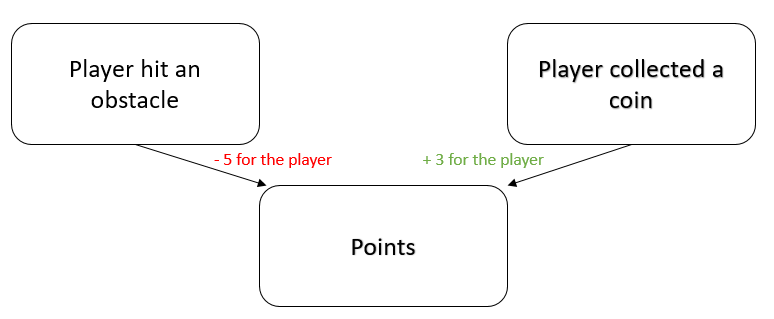
\includegraphics[width=\textwidth]{points}
    \caption{Earning and loosing point in the prototype version of the exergame}
    \label{fig:points}
\end{figure}\\
As per Figure \ref{fig:points}, the player could earn 3 points by collecting a coin. Contrarily, the player could lose 5 points if hit by an obstacle. In order to avoid hitting an obstacle or collect a coin, a movement was required to be performed by the player. Consequentially, the player was guided through the warm up routine without even realizing it. In the course of the game, the player's current score was displayed in the right corner. That way, the player had constant overview of her progress.  


\subsection{Game Scenes}


\begin{figure}[h]
    \centering
    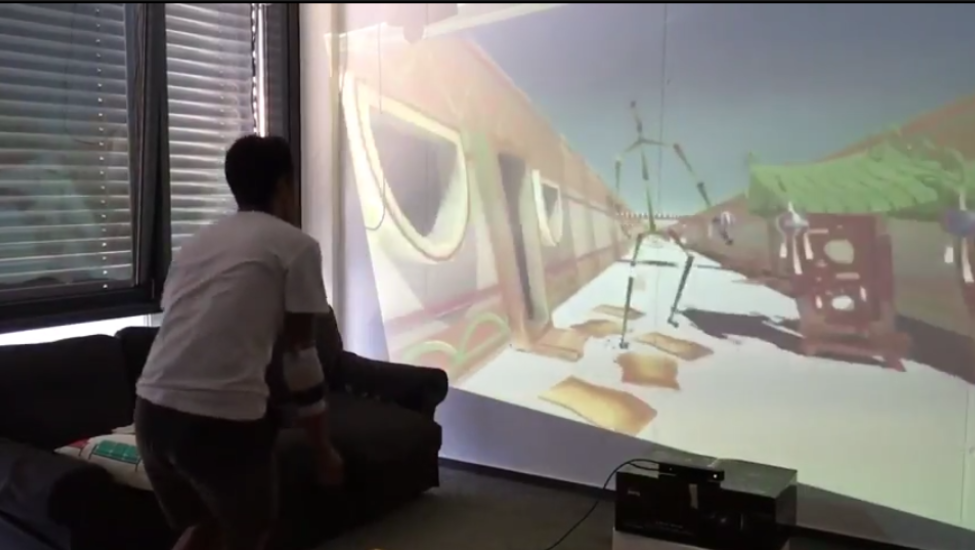
\includegraphics[width=\textwidth]{proto0}
    \caption{Earning and loosing point in the prototype version of the exergame}
    \label{fig:prototype_usage}
\end{figure}
\begin{figure}[h]
    \centering
    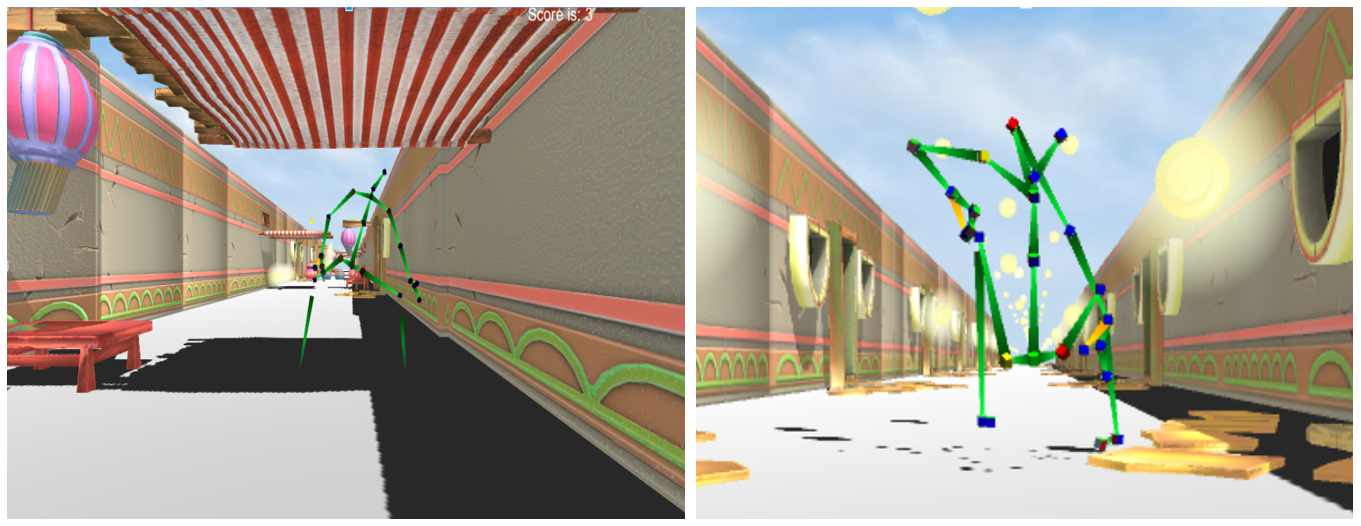
\includegraphics[width=\textwidth]{prototype}
    \caption{Earning and loosing point in the prototype version of the exergame}
    \label{fig:prototype}
\end{figure}

\section{Evaluation}
\subsection{Focus groups}
\subsection{Questionnaire}
\section{Final Exergame Solution}